\documentclass[usenatbib,fleqn]{mnras}

\makeatletter
\newlength{\abovecaptionskip}%
\setlength{\abovecaptionskip}{10\p@}
\makeatother


\usepackage{threeparttable}
 

\usepackage{amsmath,amssymb}
\usepackage{mathrsfs}
\usepackage{graphicx}
\usepackage{epstopdf}
%\usepackage{hyperref}
\epstopdfsetup{outdir=./figures/}
\graphicspath{{./figures/}}
\usepackage{url}
%\usepackage{aas_macros}

\newcommand\lsim{\mathrel{\rlap{\lower4pt\hbox{\hskip1pt$\sim$}}
    \raise1pt\hbox{$<$}}}
\newcommand\gsim{\mathrel{\rlap{\lower4pt\hbox{\hskip1pt$\sim$}}
    \raise1pt\hbox{$>$}}}

\newcommand{\Mbh}[1][]{M_{\bullet#1}}
\newcommand{\Menc}{M_{\rm enc}}
\renewcommand{\th}{t_h}
\newcommand{\Msun}{{\rm M_\odot}}
\newcommand{\pyear}{{\rm yr}^{-1}}

% write title (with email and institute)
\title{TDE jets}

\begin{document}

\begin{abstract}
  Radio light curves calculated for TDE jets. CNM
  densities based on \citet{Generozov+2015}. 
\end{abstract}
\section{Introduction}
\label{sec:intro}
When stars wander too close to a black hole (BH) they are disrupted by
tidal forces. If a star passes within a tidal radius it will be fully
torn apart with half of the material bound to the BH while the
other half is flung outwards towards infinity. It is expected that the
bound material will accrete onto the hole and create a luminous flare
\citep{Hills1975, Carter+1982, Rees1988}. 

Many tidal disruption candidates have now been identified in the
UV/optical \citep{van-Velzen+2011, Gezari+2012, Chornock+2014,
  Arcavi+2014} and/or soft x-rays \citep{Esquej+2007}. Additionally,
observers have now found three tidal disruption candidates accompanied
by synchrotron emission from relativistic outflows
(\citealt{Bloom+2011, Zauderer+2011, Cenko+2012, Brown+2015} ({\bf AG:
  should probably cite more here}). These events are all characterized
by non-thermal, highly variable x-ray emission (possibly from the base
of the jet), and self-absorbed synchrotron emission (naturally
explained by acceleration of particles at shocks formed at the
interface between the jet and cicumnuclear gas).

Although a handful of such jetted tidal disruption candidates are
now known, the overall fraction of TDEs which launches jets is small:
of order $\sim 0.1-10\%$
\citep{van-Velzen+2013}\footnote{\citet{van-Velzen+2013} give a lower
  limit of 0 in case the jetted events so far are actually associated
  with AGN activity}.  There are two classes of explanations for this:
(1) jets are launched in the majority of tidal disruption flares, but
the CNM density is either too high or too low for producing observable
synchrotron emission. (2) Jets are intrinsically uncommon. For
example, jets may be rare because the conditions required for the
Blandford-Znajek mechanism are not met in most stellar tidal
disruption events.

Here we explore the possibility that the jet emission is usually
stifled by simulating the jet-CNM interaction with a broad range of
circumnuclear medium densities. We simulate the hydrodynamic
interaction of the jet with the CNM in one and two-dimensions, and
calculate resulting synchrotron emission, as done by
\citet{Mimica+2015}. In order to isolate the effects of varying the
nuclear gas density, we fix the jet properties to the best jet model
from \citet{Mimica+2015} for the Sw J1644+57 tidal disruption flare.
This is a two component jet with a fast ($\Gamma=10$) core and a slow
($\Gamma=2$) sheath with isotropic equivalent energy $E=4 \times
10^{54}$ ergs {\bf AG--Modification for reproducing 2-d sims...}.

To establish low and high density limits for the circumnuclear gas, we
consider the rate of mass injection from stellar winds for different
stellar populations. A younger stellar population would have
significant wind mass loss from O \& B stars. In contrast, these rate
of wind mass loss from an older population, which lacks these massive
stars, could $\sim 2$ orders of magnitude smaller. We use the
formalism of \citet{Generozov+2015} (hereafter GSM15) to estimate CNM
gas density for a broad range of stellar populations. By comparing the
radio light-curves with observed radio upper limits, we test whether
TDE jets would produce observable synchrotron emission for the
physically expected range of CNM densities.

The remainder of the this paper is organized as follows: In
$\S\ref{sec:cnm}$ we bracket the range of physically expected CNM
densities. In $\S\ref{sec:jet}$ we describe the our model for the TDE
jet and the jet-CNM interaction. We use both 1d and 2d hydrodynamic
models to simulate the jet propagating through the CNM and compare the
results in $\S\ref{sec:2d}$. In $\S\ref{sec:results}$ we show radio
light-curves from our 1d models for a wide range of CNM densities, to
illustrate qualitatively how much varying the CNM density by itself
could change the radio light-curve.  We discuss the implications of
our models for detections of TDEs by future radio surveys in
$\S\ref{sec:disc}$, and summarize our conclusions in
$\S\ref{sec:conc}$.

\section{CNM density}
\label{sec:cnm}

\subsection{Model}

The density profile of the CNM encountered by a relativistic TDE jet
will affect the observed radio light curve. A very high density could
rapidly decelerate the jet, suppressing the synchrotron emission. A
very low density would gradually decelerate the jet and spread the
radio emission over long time scales \citep{Mimica+2015} {\bf but this
is not what we actually see in the simulations}.  It could be 
radio emission from TDE jets is only observable for a narrow range of
CNM properties. Although the empirical rate of jetted tidal disruption
events is small (0.1-10\% of the TDE rate according to
\citealt{van-Velzen+2013}) it is possible that the intrinsic rate is
far higher.

We calculate radio light curves for a range of physically plausible
CNM densities, to explore what conditions are required for TDE jets to
produce observable radio emission. 

The dominant source of gas injection into the CNM of quiescent
galaxies is winds from stars in the galactic nucleus. The 1D spherical
hydrodynamic equations with stellar wind mass injection are
(e.g. \citealt{Holzer+1970}) {\bf AG: possibly the detailed
  description of the CNM model should get a separate appendix.}


\begin{align}
  &\frac{\partial \rho}{\partial t}+\frac{1}{r^2}\frac{\partial}{\partial r}\left(\rho r^2 v\right)=q \label{eq:drhodt}\\
  &\rho \left(\frac{\partial v}{\partial t} + v\frac{\partial
      v}{\partial r}\right) =-\frac{\partial p}{\partial r}- \rho\frac{GM_{\rm enc}}{r^{2}} -q v \label{eq:dvdt}\\
  &\rho T\left(\frac{\partial s}{\partial t} + v\frac{\partial
      s}{\partial
      r}\right)=q\left[\frac{v^2}{2}+\frac{v_w^2}{2}-\frac{\gamma}{\gamma-1}
    \frac{p}{\rho} \right] ,
\label{eq:dsdt}
\end{align}

where $\rho$, $v$, $p$, and $s$ are the density, velocity, pressure, and
specific entropy, respectively.  $\Menc$ is the combined black hole
and enclosed stellar mass. The pressure is given by an ideal gas
equation of state.  {\bf AG: Quick summary of previous work on
  modeling CNM density.}

 {\bf AG: note I took the mean molecular weight to be
  0.62.}

$q$ is the mass injection rate per unit volume per unit time and is
proportional the stellar density divided by a Hubble time: $q=\eta
\rho_\star/\th$. $v_w$ encapsulates the heating of the gas. Physically
this may come from (1) the stellar wind kinetic energy (2) supernovae
(3) black hole feedback.

\citet{Generozov+2015} find that the gas density depends on the
mass return parameter, $\eta$, the heating rate, $v_w$, the black hole
mass, $\Mbh$, and the power law slope of the stellar density profile
($\rho_\star\sim r^{-\delta_1}$ for small radii).

For a cusp galaxy ($\delta_1> 0.5$), the gas density, $\rho\sim
r^{-1}$. In this case the gas density at $10^{18}$ cm, $n_{18}$ can be
approximated using a simple scaling relation 

\begin{equation}
n_{18}\simeq 0.4 \Mbh[,7]^{0.5} \eta_{0.02} v_{500}^{-1.5} {\rm
  cm^{-3}},
\label{eq:n18}
\end{equation}

where $\Mbh[,7]=\frac{\Mbh}{10^7 \Msun}$,
$\eta_{0.02}=\frac{\eta}{0.02}$, and $v_{500}=\frac{v_w}{500 {\rm
    km/s}}$, and we have assumed a fixed slope for the stellar density
power law slope $\delta_1=1.8$. Thus, the gas density is quite
sensitive to the mass return parameter and the heating rate, which are
related to the star formation history. Young, massive stars put out
very energetic winds with $v_w\simeq 1000$ km/s with a high mass
return rate, $\eta\simeq 100$, in contrast stars with age comparable
to hat of the universe will have slow winds with speeds of order $\sim
10$ km/s and mass return parameters, $\eta\simeq0.02$. In the next
section we explore the range of mass return parameters, heating rates,
and gas densities allowed by plausible star formation histories.

\subsection{Plausible range of CNM gas densities}
Increasing the mass return parameter, $\eta$, or decreasing the
heating parameter $v_w$, increases the gas density, $n_{18}$.
However, one cannot increase the $\eta$ or decrease $v_w$ arbitrarily
as the CNM will become thermally unstable. Specifically if the heating
rate falls below

\begin{equation}
v_{\rm w,TI}\simeq 200 \eta_{0.02}^{0.17} \Mbh[,7]^{0.08} \,{\rm km/s} 
\label{eq:ti}
\end{equation}

{\bf AG: for vw$>1000$ km/s the cooling will be dominated by
  Bremstrahlung and so the ti criterion may be somewhat different} If
the heating rate falls below this critical value the CNM will become
thermally unstable, condensing into cold clouds {\bf
  AG--caveats}. Thus, the maximum possible density $n_{18}$ for a
given $\eta$ will correspond to $v_{\rm w,TI}$. From
equations~\eqref{eq:n18} and~\eqref{eq:ti} this will be given by

\begin{equation}
n_{\rm 18,TI}\simeq 1.6 \eta_{0.02}^{0.75} \Mbh[,7]^{0.38} \, {\rm cm^{-3}}
\label{eq:n18ti}
\end{equation}

The maximum physical $\eta\simeq 400$\footnote{For details
  of how to calculate $\eta$ for a given star formation history see
  appendix C of \citet{Generozov+2015}.} occurs $\sim 3$ Myr after a
burst of star formation. Evaluating equation~\eqref{eq:n18ti} with
$\eta=400$ gives the maximum possible CNM density

\begin{equation}
n_{\rm 18,max} \simeq 2,700 \Mbh[,7]^{0.38} {\rm cm^{-3}}
\label{eq:n18max}
\end{equation}

Although such large gas densities would be present in the immediate
aftermath of a starburst, the wind mass loss rate (and thus the gas
density) declines as $\eta \sim t^{-3}$. Thus we expect the gas density would
decline by an order of magnitude after a few Myr. Note that type II
Supernovae could inject additional mass into the CNM, but this
injection would be intermittent (e.g. the time between SNe would be
long compared to a dynamical time).

However, we also find high gas densities ($n_{18}\sim 2000$ cm$^{-3}$)
may be present for E+A galaxies with stellar ages $\tau_\star\sim
10^8-10^9$ years. Although E+A galaxies are rare they host $\sim 20
\%$ of all optically selected TDE candidates. Thus, the high density
limit could be relevant for a sizable fraction of TDEs {\bf AG citation
  needed here...}

{\bf AG too much detail?} We construct a gas density profile for the
nearby E+A galaxy NGC 3156. This galaxy has a stellar light profile
measured with high resolution HST photometry. \citealt{Krajnovic+2013}
find a steep inner stellar density profile with $\rho_\star\sim
r^{-2.78}$, albeit with a possible turnover to a shallower profile at
$r \sim 2-4$ pc. We assume a core-like profile with $\rho_\star \sim
r^{-1.1}$ for $r<2$ pc.

We find a thermally stable profile for NGC 3156 for mass
return parameter $\eta\simeq0.5$ and Type Ia supernova heating
$v_w\simeq600 $ km/s, as expected for 1 Gyr after a burst of star
formation. We find $n \sim 2000 (r/10^{18} {\rm cm})^{-1.3}$
cm$^{-3}$, for $r<2$ pc, $n\sim r^{-2}$ for $r>2$ pc, which is quite
similar to the profile for a normal cusp galaxy with break at $r_b$=2
pc. {\bf AG--w/o turnover the inner density slope would be -2--possibly
do a special case?}

Such a large gas density should produce a large x-ray luminosity in
the galactic nucleus from metal line cooling and free-free emission.
In particular our model for the E+A galaxy predicts an x-ray
luminosity of $\sim$ few $\times 10^{39}$ egs/s, from the inner few
parsecs of the galaxy {\bf AG--reran with proper normalization of the
  cooling function (this was incorrect in GSM15). Would be good to
  double-check these results.}


We found an archival X-ray observation from ROSAT for this galaxy {\bf
  AG describe observation here; look for other observation}. There are
no X-ray sources consistent with the galactic nucleus, which gives a
90\% confidence of upper limit $<2.4$ counts over the $\sim$400 s
exposure time. We then use this non-detection to put an upper limit on
the unresolved x-ray flux from the galactic nucleus using the
web-PIMMS
tool\footnote{https://heasarc.gsfc.nasa.gov/cgi-bin/Tools/w3pimms/w3pimms.pl}. We
use an APEC emission model, temperature of ($10^{7} K$--the
approximate temperature of the gas for radii dominating the x-ray
emission a solar metallicity ({\bf AG Check for metallicity
  measurements for this galaxy}), and $2.43\times 10^{20} {\rm cm^{-2}}$ for
the galactic HI column density\footnote{from https://heasarc.gsfc.nasa.gov/cgi-bin/Tools/w3nh/w3nh.pl}. With
these parameters non-detection gives an upper limit on the flux of
$\lsim 2\times 10^{39}$ ergs/s {\bf AG check for other x-ray
  images}. Thus, the non-detection is marginally consistent with the
model, though it shows the density cannot be much higher than we
predict.

What is the smallest plausible CNM density? This would correspond to a
small mass return parameter and a high heating rate. The mass return
parameter, $\eta=0.02$, reaches its minimum value for a stellar
population that is a Hubble time old. A stellar population
that is $<$ 3 Myr old will have a heating rate, $v_w=3,000$ km/s.

A stellar population in which a small fraction, $f$ of the stars
formed $\lsim 3$ Myr ago and the rest are a Hubble time old, will have
both a high heating rate and a low mass return rate. In this scenario
$n_{18}$ will be minimized for $f=4\times 10^{-4}$. Both old and young
stars contribute significantly to the mass injection rate giving
$\eta\simeq 0.03$, while the young star dominate the heating
$v_w\simeq 3,000$ km/s and thermally stabilize the gas. These
parameters give us the minimum possible CNM gas density

\begin{equation}
n_{\rm 18,min}\simeq 0.06 \Mbh[,7]^{0.5} {\rm cm^{-3}}
\label{eq:n18min}
\end{equation}

We illustrate how the mass return parameter, heating rate, and
density vary with star formation history in Fig.~\ref{fig:param}. The
gray lines represent a two-burst model for star formation in which a
fraction, $f$, of the stars formed $<$ 3 Myr ago and the remainder
formed a Hubble time ago (top gray line) or 1 Gyr ago (bottom red
line).  Towards the top right the $f=1$ and the young stars dominate
the mass injection rate and the heating rate.  Moving towards the
left, $f$ decreases, along with the mass return rate, and density
(blue lines), but the heating rate, $v_w$, remains $\gsim 1000$ km/s
except for very small values of $f$. The bend in the top, solid, gray curve
corresponds to the minimum possible CNM density.

The dashed, gray line also represents a two burst formation history
but the older burst is $\sim 3$ Myr old (right at the age when stars
are beginning to leave the main sequence, increasing the mass
injection rate. Towards the lower right of the dashed, gray line these
somewhat older stars dominate the mass injection into the CNM,
increasing the density past the thermal instability threshold (thick,
black line). The intersection between the dashed gray line and the
thermal instability line corresponds to the maximum possible CNM
density.

\begin{figure} 
  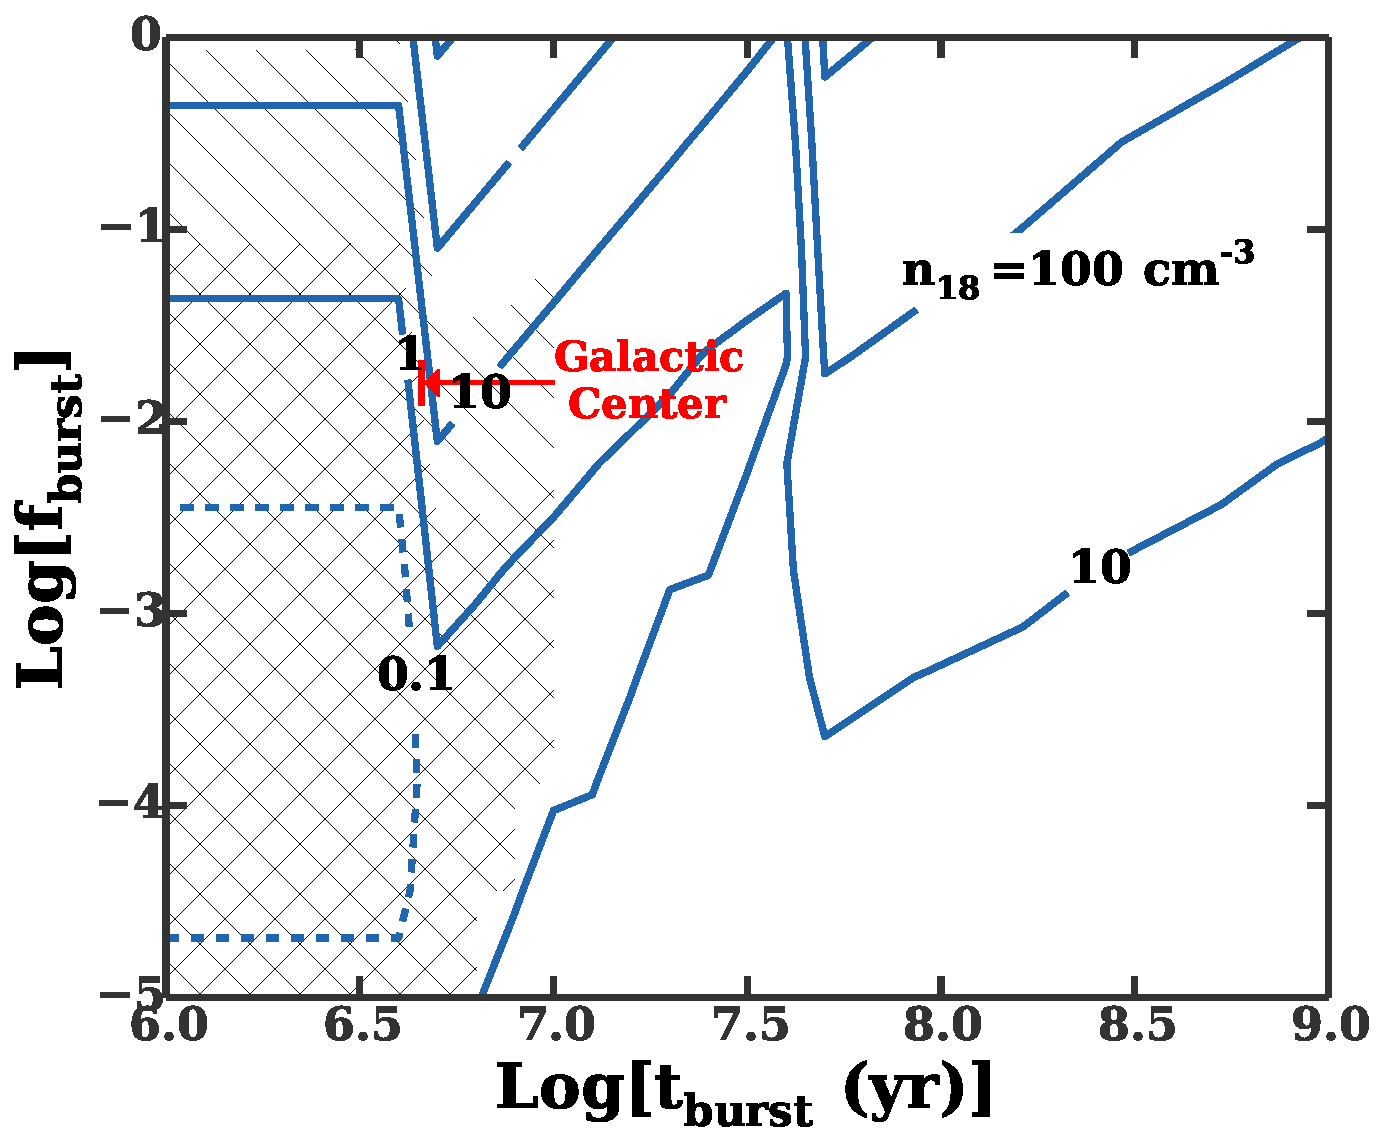
\includegraphics[width=8cm]{cnm_plot.pdf}
  \caption{\label{fig:param} Heating rates ($v_w$) and mass return
    parameters ($\eta$) for different star formation histories (gray
    lines). Solid, gray lines correspond to a star-burst of $<3$ Myr
    ago forming a fraction $f$ of the stars. The rest of the stars
    formed either a Hubble time ago (top line) or 1 Gyr ago (bottom
    line). The fraction $f$ increases and the gas density from left to
    right along these lines. The dashed, gray line corresponds to an
    alternate scenario in which there are two recent bursts in rapid
    succession in rapid succession: the older burst is $\sim 3$ Myr
    old (just at the point when stars are beginning to leave the main
    sequence). The contribution of this older burst increases towards
    the right, crossing boundary of the thermally unstable (``TI'')
    region below the thick black line.}
\end{figure}


\subsection{Alternative constraints on CNM gas density}
In this section we present alternative constraints on the CNM gas
density.  

\citet{Heckman+2004} find that in the local universe small black
holes {\bf (AG $\Mbh\sim 10^6 \Msun$?)} have growth times, $t_{\rm grow}$
comparable to a Hubble time, $t_h$, while massive black holes have
$t_{\rm grow} \gg \th$. This can be used to put a constraint on the
black hole accretion rate, $\dot{M}_{\bullet}$:

\begin{align}
\dot{M}_{\bullet} &\lsim \frac{\Mbh}{t_h} \lsim 7 \times 10^{-4}
\Mbh[,7] \,\, \Msun \pyear
\label{eq:tgrow}
\end{align}

The black hole accretion rate is some fraction $f_{\rm in}<1$ of the
large scale inflow rate $\dot{M}$. So equation~\eqref{eq:tgrow} can be
translated into an upper bound for gas density, $n_{18}$, using
$\dot{M}_{\bullet} = f_{\rm in} \dot{M} = f_{\rm in} 4 \pi r^2 \mu m_p
n v$.  Assuming an inflow velocity $v=\sqrt{G M/r}$ {\bf AG double
  check this equation.}

\begin{align}
n_{18} &\lsim 10^3 \Mbh[,7]^{0.5} \left(\frac{f_{\rm in}}{0.1}\right)^{-1}
{\rm cm^{-3}}, 
\label{eq:tgrowDens}
\end{align}

e.g. within a factor of a few of the high density limit given in
equation~\eqref{eq:n18max}, for $f_{\rm in}$=0.1. However, we note
that the value of $f_{in}$ is a large source of uncertainty in this
analysis. In our own galaxy Faraday rotation measurements {\bf AG
  cite!} suggest $f_{in}\simeq 0.001$.

An alternative constraint may be derived by considering the effects of
black hole feedback. Equation 45 in GSM15 provides an expression for
the inflow rate for which Compton heating self-regulates the accretion
flow:

\begin{align}
\frac{\dot{M}_{C}}{\dot{M}_{\rm edd}} \approx 
% \Begin{cases} 2\times 10^{-3} \eta_{0.02}^{0.2}T_{\rm
% C,9}^{-0.8}\epsilon_{-2}^{-0.8} M_{\bullet,8}^{0.16}
% &, \text{core}\\
8\times 10^{-4} \eta_{0.02}^{0.3}T_{\rm
C,9}^{-0.7}\epsilon_{-2}^{-0.7} M_{\bullet,8}^{0.14}
&, \text{cusp}, 
  \label{eq:MdotCa}
\end{align}

where $\epsilon_{-2}=\epsilon_{\rm rad} f_{\rm in}/0.01$, depends on
both ratio of the accretion rate to the large scale inflow rate,
$f_{\rm in}$, and the radiative efficientcy of the inner accretion
$\epsilon_{\rm rad}$, which is itself a function of the accretion
rate. $T_{C,9}$ is the Compton temperature normalized to $10^9$
K (see...). Taking $\epsilon_{\rm rad}=0.03$ and the maximum physically
plausible $\eta=400$, we obtain

\begin{align}
n_{18} \simeq 700 \Mbh[,7]^{0.6} \left(\frac{f_{\rm
      in}}{0.1}\right)^{0.7} \left(\frac{T_{\rm C}}{10^9 {\rm
      K}}\right)^{-0.7} {\rm cm^{-3}},
\end{align}

{\bf AG note that the maximum physically plausible eta already
  presupposes that the mass budget is dominated by young stars, and in
this regime we expect that Compton heating would be very
subdominant...}

{\bf AG momentum based feed-back.}


{\bf AG Jeans criterion -- but be careful of tidal effects.}

AGN feedback would may blow low density bubbles in the
CNM. \citet{Russell+2013} used Chandra x-ray observations to measure gas
density and temperature profiles for a sample of massive elliptical
galaxies. The measured electron density on scales of $\sim 100
pc$ is $\gsim 0.1$ cm$^{-3}$. Note that the gas density at 100 pc
would be irrelevant for a TDE jet, but we would not expect the gas
density to be decreasing towards the galactic center in a steady
state. {\bf These are only massive ellipticals with $\Mbh\sim 10^{9} \Msun$.}

\subsection{Adopted gas density profiles}
 The following density provided a good fit to the CNM density profile
 of cusp galaxies.

\begin{align}
n=
\begin{cases}
  n_{18} \left(\frac{r}{10^{18} {\rm cm}}\right)^{-1} {\rm cm^{-3}} & r<r_b \\
  n(r_b) \left(\frac{r}{r_b}\right)^{-\beta} {\rm cm^{-3}} & r\geq
  r_b,\\
  \label{eq:profile}
\end{cases}
\end{align}

where $0.1 \Mbh[7]^{1/2} \lsim n_{\rm 18}\lsim 2,700
\Mbh[7]^{0.38} $ cm$^{-3}$.  

The gas density density experiences a break at radius $r_b$, the break
radius in the stellar density profile, where the stellar density
transitions from an inner power law slope $\delta_1\lsim 2$ to an outer
power law slope $\delta_2\gsim 2$. $r_b\gsim 100$ pc for cusp galaxies,
in which case the break radius may be safely ignored as it will be
well outside the jet deceleration radius. If there is a nuclear
star cluster present the effect $r_b$, the outer boundary of the
nuclear star cluster will correspond to a much smaller effective
$r_b\sim 1-5$ pc. However, even in this case the break radius is still
one too large scales to affect the light-curve evolution {\bf AG why?}
Thus, we don't include a break radius in our gas density profiles.

We perform simulations with CNM density $n=n_{18} \left(r/10^{18} {\rm
  cm}\right)^{-1}$ with $n_{18}$=2, 60, and 2000 to see what effect
varying the CNM density would have on the observed radio light-curve.

% The outer power law slope of the gas density will depend on the slope
% of the $\beta$ but will typically vary between 1.5 and 2. 

% We explore the parameter space of $n_{18}$, $\beta$, and $r_b$,
% adopting values for these parameters summarized by
% Table~\ref{tab:params} below


% \begin{table}
%   \caption{\label{tab:params} Summary of numerical parameters used for
%     the CNM profile (equation~\eqref{eq:profile}). A ``-'' in the $r_b$
%     or $\beta$ columns indicates that the gas density profile is a
%     single power law without any breaks. ``...'' in any column
%     indicates the entry is the same as the one above it.}
% \begin{minipage}{\columnwidth}
% \begin{tabular}{|l|l|l|}
% $n_{18}$ & $r_b [{\rm pc}]$ & $\beta$\\
% \hline
%   2     &  -    &  -\\
%   60    &  -    &  -\\
%   ...   &  1    &  1.5\\
%   ...   &  ...   &  2\\
%   2000  &  -    &  -\\
% \end{tabular}
% \end{minipage}
% \end{table}


{\bf AG cores...}

We also use a core galaxy profile to see how the shape of the stellar
density profile would affect the radio lightcurve. For core galaxies
the stellar density profile is not a pure power law. To simplify
things we will consider one particular slope for the stellar density
profile: $\rho_\star\sim r^{-\delta_1}$ with $\delta_1=1.1$. The gas
density profile may be approximated as

\begin{align}
\begin{cases}
n=n(r_s) k(x) & 0.4 \leq x\leq 2.0\\
n = 2.0 n(r_s) (x/0.4)^{-0.95} & x < 0.4\\
n = 0.75 n(r_s) (x/2.0)^{-0.26} & 2.0< x \leq r_s/r_b\\
n \sim x^{-1.5} & x>r_s/r_b\\
\end{cases}
\label{eq:cores}
\end{align}

Where, 

\begin{align}
  &x=r/r_s\\\nonumber
  &k(x)=\frac{45}{19} \frac{1}{x^{3/2}} \frac{1-x^{1.9}}{9-19
      x\frac{x^{0.9}-1}{x^{1.9}-1}}
\end{align}

To isolate the effects of the shape of the density profile, consider a
core density profile with $r_s=10^{18}$ cm, and $n_{18}=2000$: the
same as our high density cusp model.

% We consider a high density model (near the verge of thermal
% instability) and a low density model (near the lower limit of what
% stellar winds can give for the CNM density). The values $n(r_s)$ and
% $r_s$ are given in the table below. 

% \begin{table}
% \begin{tabular}{|l|l|l}
%  core models & $n(r_s)$ & $r_s$\\
% \hline
%  High & 2,500 $\Mbh[7]^{-0.32}$ cm$^{-3}$ &  4 $\times 10^{17}  
%  \Mbh[7]^{0.8}$ cm\\
%  Low & 0.1 $\Mbh[7]^{-0.24}$ cm$^{-3}$ & 6$\times 10^{16} \Mbh[7]$ cm
% \end{tabular}
% \end{table}

\section{TDE jets}
\label{sec:jet}
This section would summarize modeling of TDE jets.

\subsection{Jet Models}

\subsection{Hydrodynamics}

\subsection{1-d vs. 2-d Models}
\label{sec:2d}
We compare the light-curves for 1-d and 2-d jet simulations with the
same structure (fast ($\Gamma=10$) core and slow ($\Gamma=2$)
sheath). Note that the hydrodynamic evolution of these 2 components is
independent in 1-d, but the radiative transfer/light-curve calculation
is sensitive to the jet geometry.

2-d effects reduce peak radio luminosity, especially for large
observing frequencies and on-axis jets. Two-dimensional jets also show
an earlier peak for off-axis events (see Fig.~\ref{fig:1d2d}).

\begin{figure}
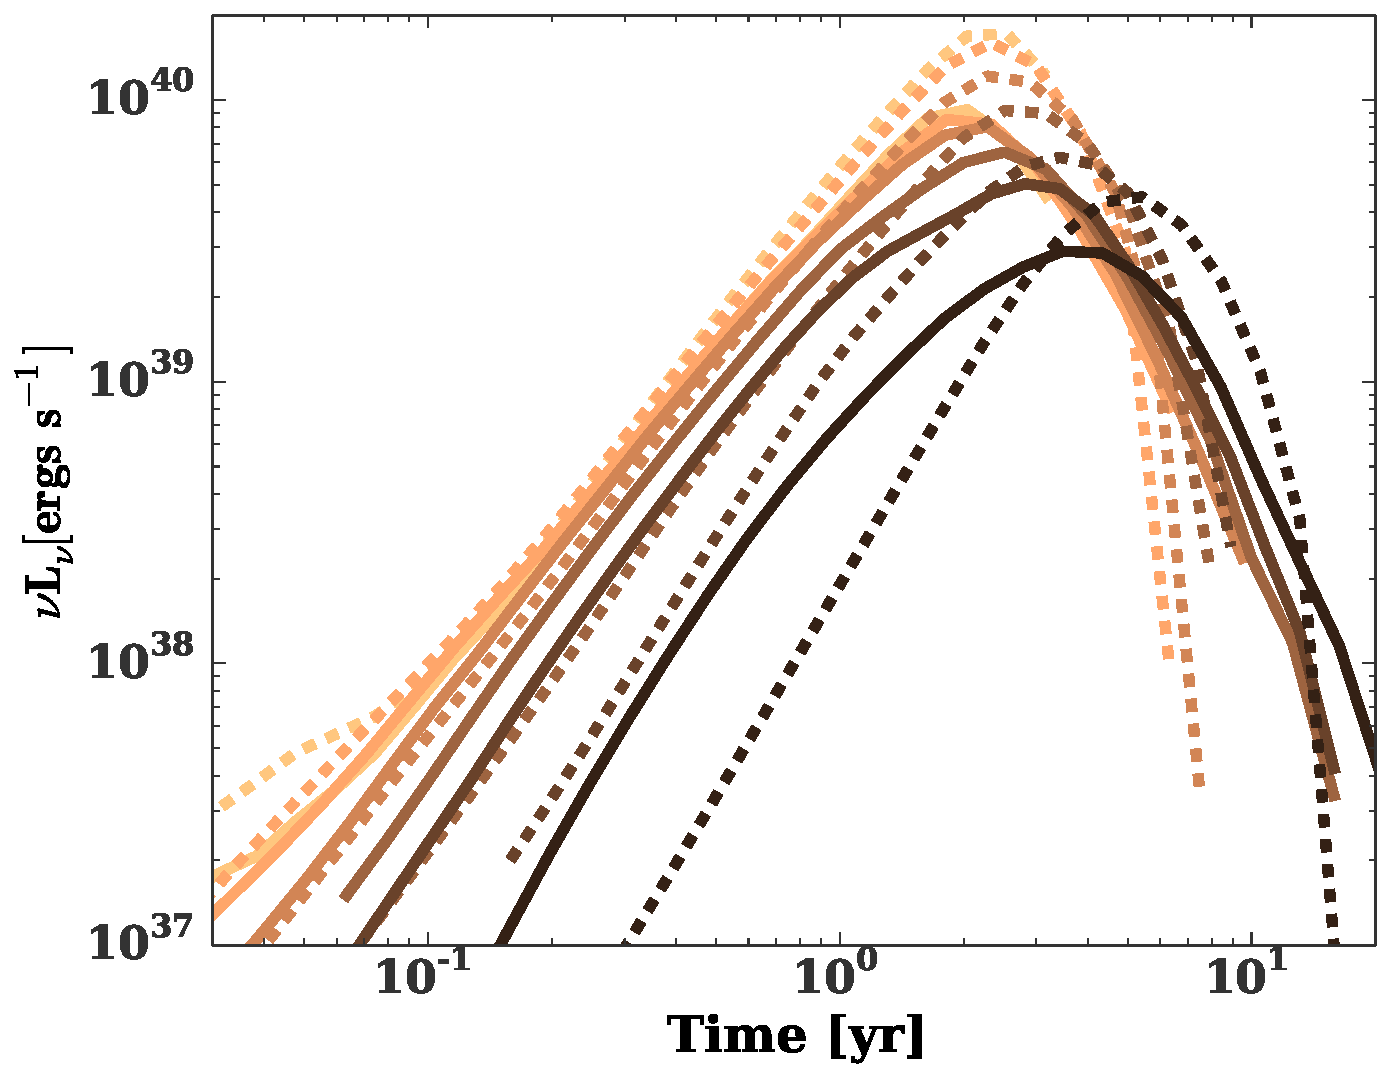
\includegraphics[width=8cm]{comparison_1ghz.pdf}
\caption{\label{fig:1d2d} Comparison of 1-d (dashed) and 2-d (solid)
  light-curves for 1 GHz, for fixed CNM density $n=60
    (r/10^{18} {\rm cm})^{-1}$. {\bf AG--2d simulations are actually
      performed with an -1.5 profile. 4 pi correction}}
\end{figure}

These discrepancies are due to the fact that in 2-d the jet rapidly
spreads out and becomes quasi-spherical {\bf AG--dependence on
  density.} 

For the 1-d models we calculate a spherical blast wave, which has the
same energy as the jet within the assumed opening angle (0.5 radians).
Thus, the simulated isotropic blast wave is much greater than the energy of
the jet. This would be appropriate for a jet with a constant jet
opening angle.

In reality, we see that the jet expands laterally, so that at
sufficiently late times the expansion becomes quasi-spherical in the
2-d simulations.

We find that to a good approximation the results of two component 2-d
simulations may be reproduced using a 1-d simulation with the same
fast core, and a slow component spread over all other solid angles
(``istoropized''), with the same energy as in the 2-d simulations.  We
show a comparison of this modified 1-d approach, with the true 2-d
result in Figure~\ref{fig:1d2dB}, for $n_{18}=60$ and $n_{18}=2000$.
Based on this excellent agreement, we will from now one use
  isotropized 1-d models to produce radio light-curves light-curve.

\begin{figure*}
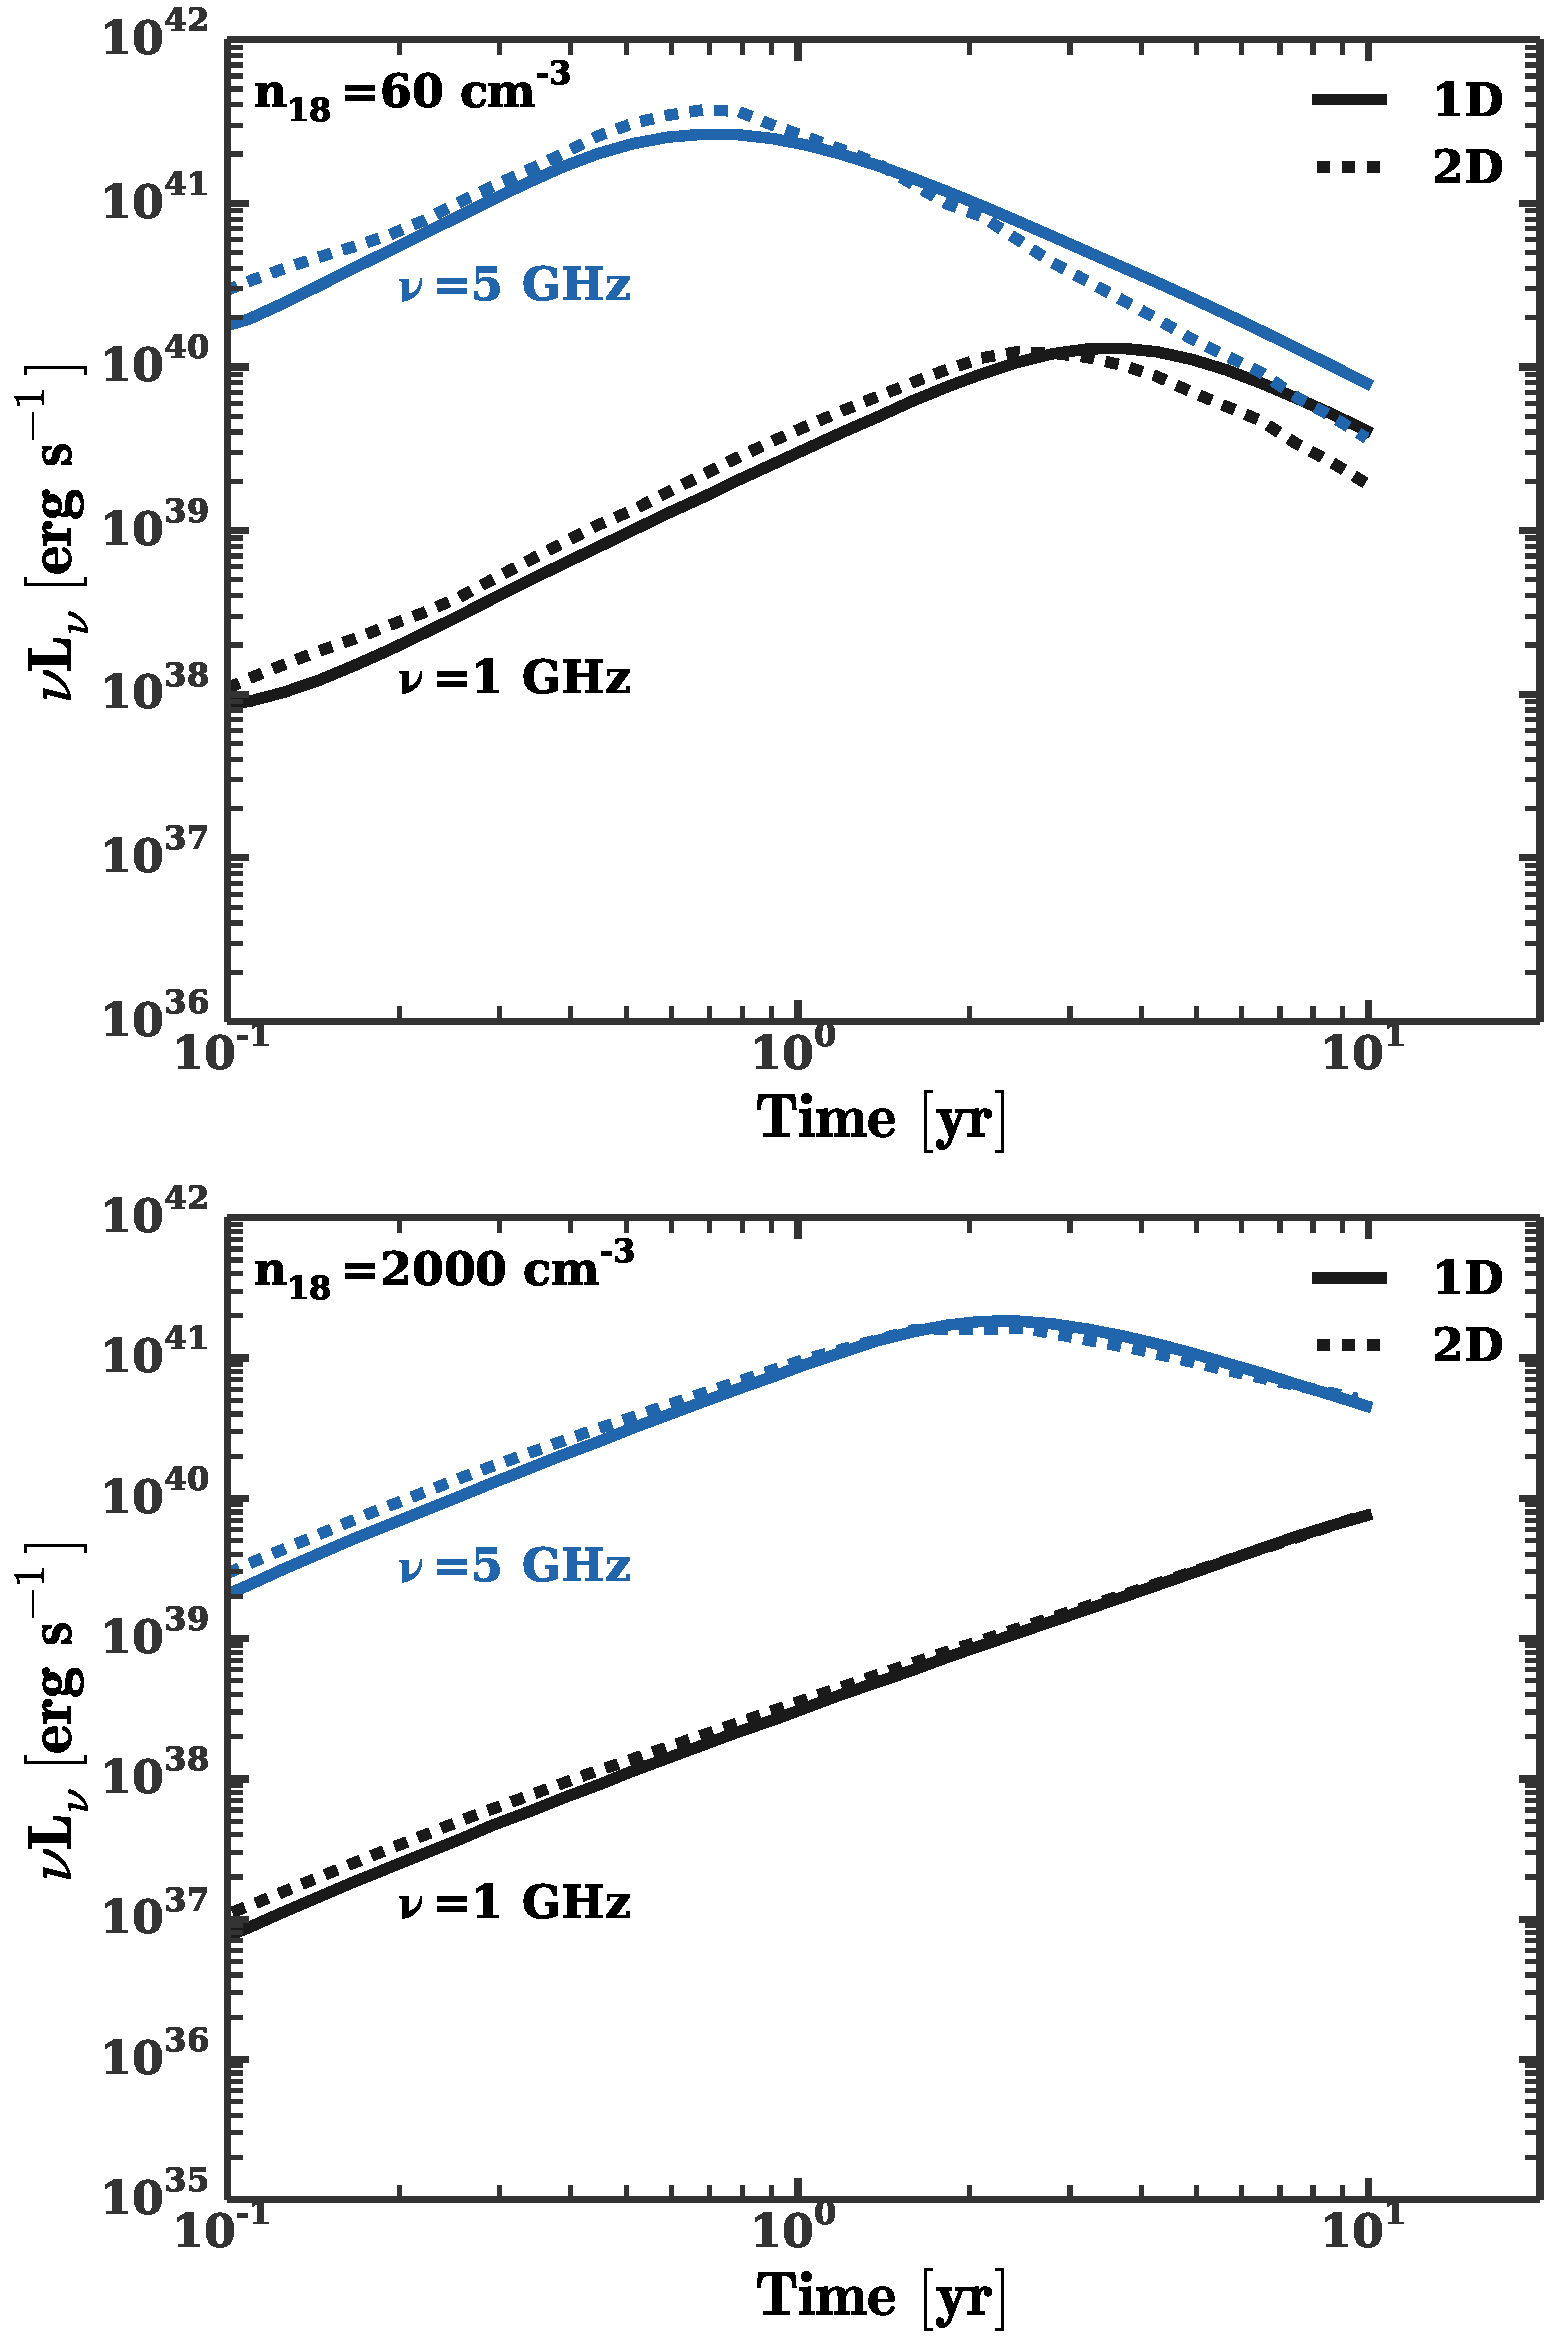
\includegraphics[width=16cm]{1d_2d.pdf}
\caption{\label{fig:1d2dB} Comparison of on-axis light-curves for
  $n_{18}=60$ (top) and $n_{18}=2000$ (bottom) for frequencies of 1
  GHz (left) and 30 GHz (right). For the 1d simulations here we reduce
  the isotropic equivalent jet energy by a of eight compared to
  figure~\ref{fig:1d2d}, to account for the lateral spreading of the
  jet. We assume an $n\sim r^{-1}$ density profile for $n_{18}=2000$, but
  take $n\sim r^{-1.5}$ for $n_{18}=60$ for computational convenience.}
\end{figure*}


\section{Results}
\label{sec:results}

\subsection{Effects of gas density}

In Fig.~\ref{fig:upper_limits} we show the on-axis light curves for
our fiducial jet model and CNM density profile $n=n_{18} (r/10^{18}
{\rm} cm)^{-1}$ cm$^{-3}$ with $n_{18}$=2, 60, and 2000 cm$^{-3}$. The
higher density models peak at later times with smaller peak
luminosities {\bf AG Do we understand this? Is this due to the effect
  of self-absorption?}

{\bf AG it would probably be good to have a figure showing the
  different components contributing to the emission.} The radio light
curve has contributions from both the slow and fast jet
components. The fast component dominates at
early times for the $n_{18}=2$ and 60 lightcurves, while the slow
component dominates for all times as frequencies for
$n_{18}$=2000. Generally, the fast component is more important at
higher frequencies, and lower densities.

We also show radio upper limits and detections for various TDE
candidates in Fig.~\ref{fig:upper_limits} (these were compiled from
various sources into Table 1 of \citealt{Mimica+2015}). Overall, the
measurements were taken too late to be strongly constraining,
especially for the low density models: the lightcurves or $n_{18}=2$
peak on time-scales of months, while many of the radio measurements
were taken decades after the TDE flare.

\begin{figure} 
  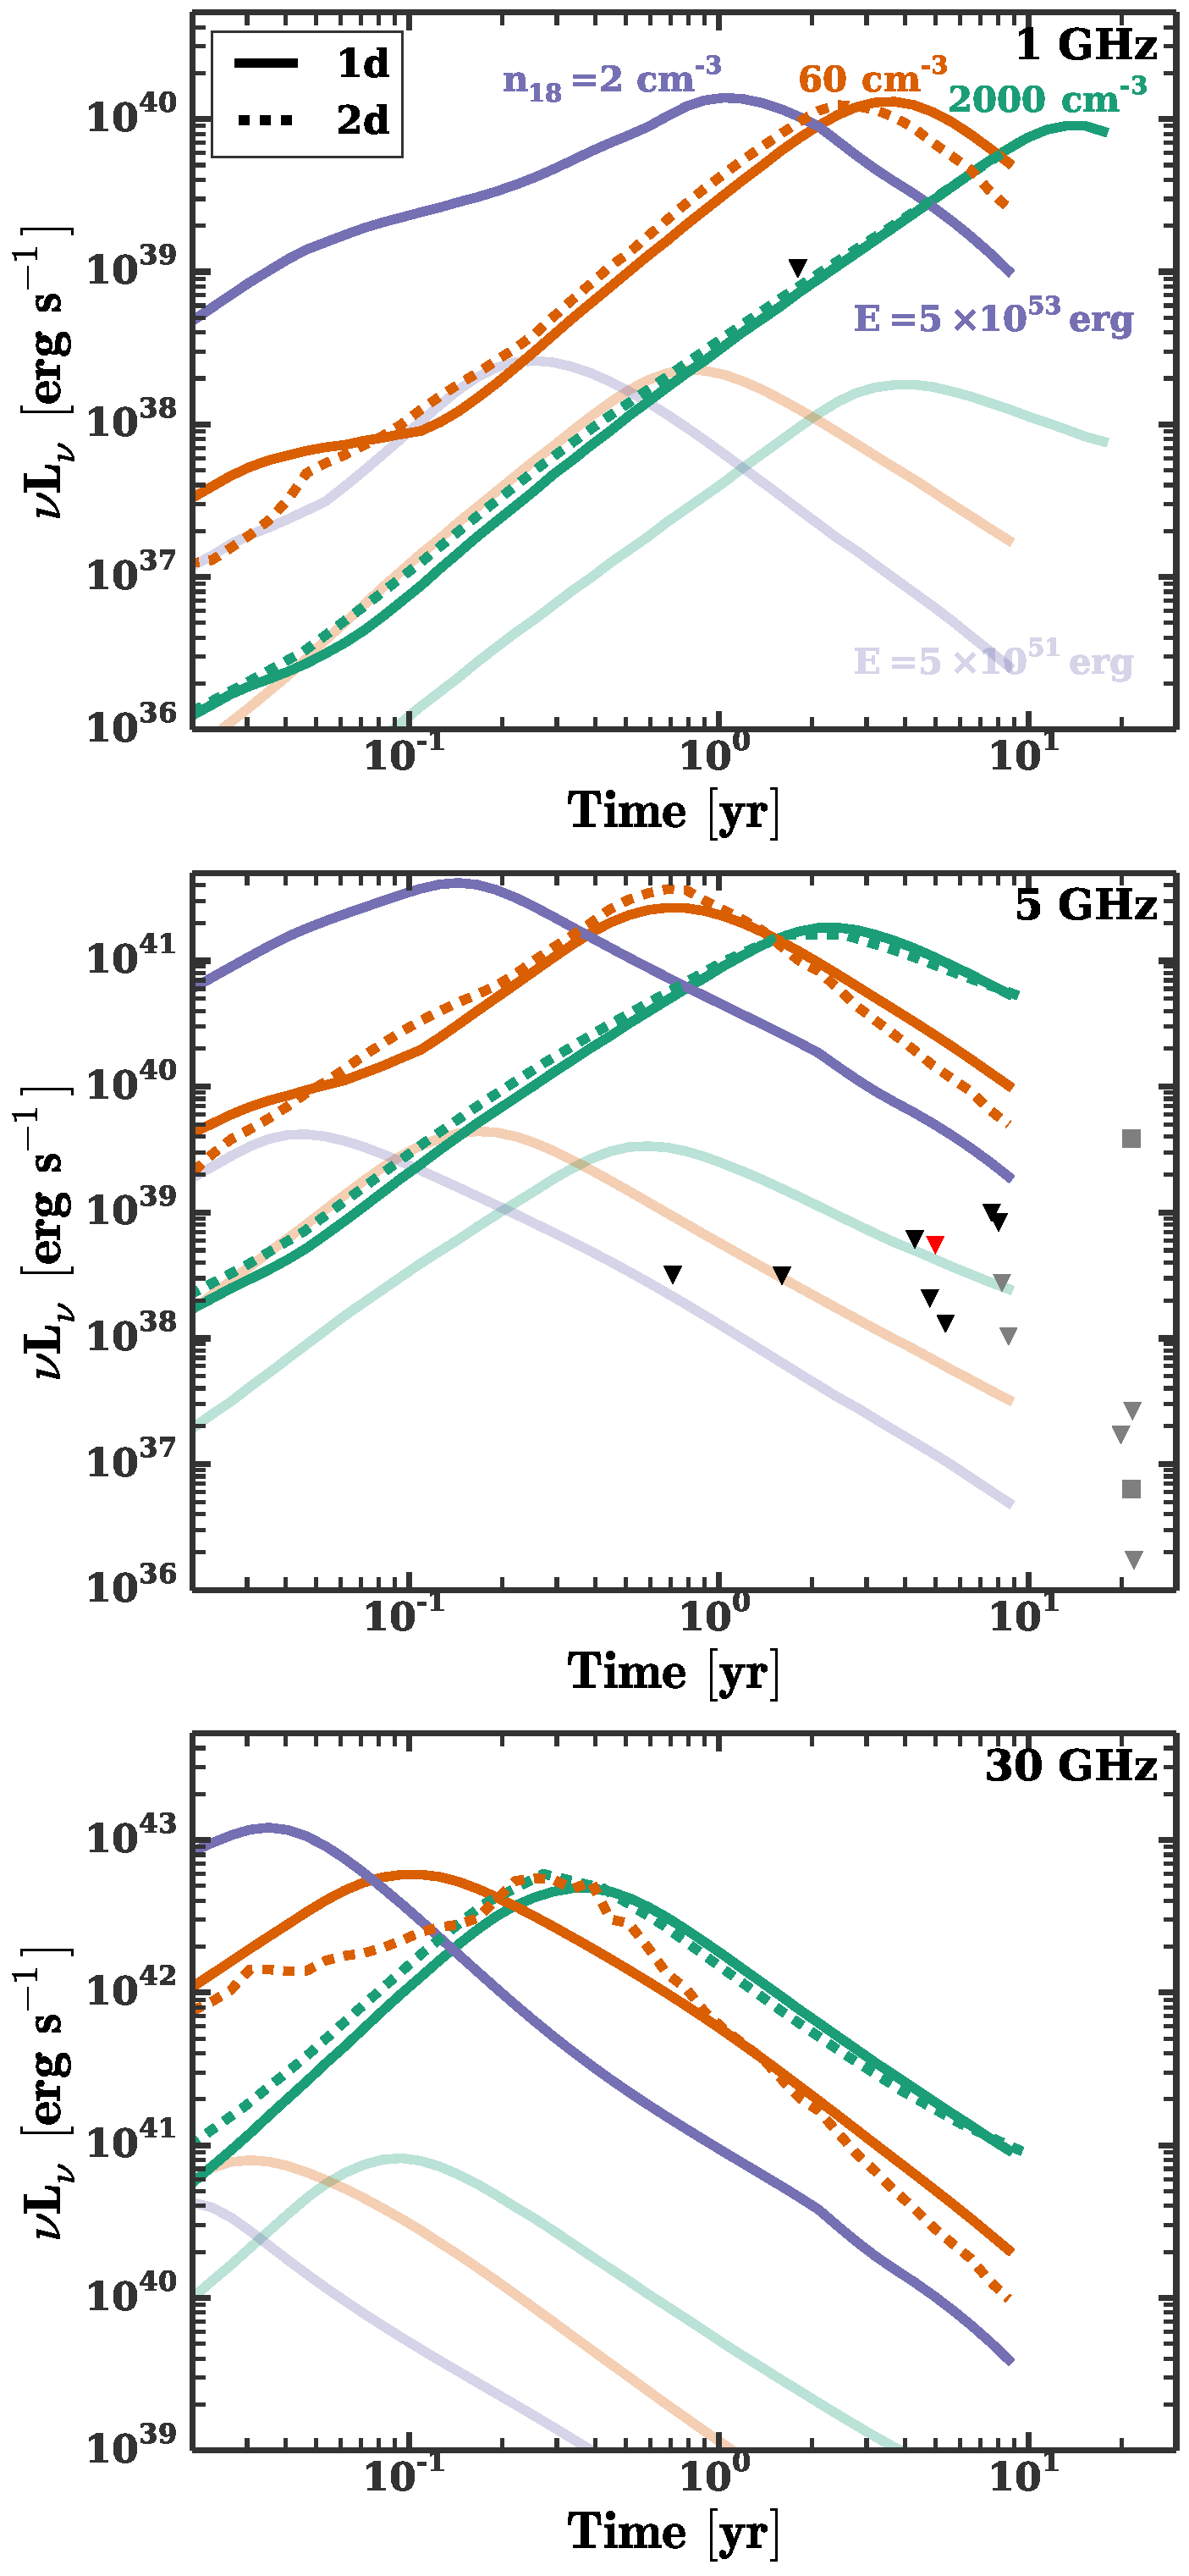
\includegraphics[width=8cm]{lightcurves.pdf}
  \caption{\label{fig:upper_limits} On-axis radio light-curves for
    fiducial jet model ({\bf AG-Summary table for jet models}) and CNM
    density profile $n=n_{18} (r/10^{18} {\rm cm})^{-1}$, for three
    different values of n$_{18}$: 2, 60, and 2000. Radio upper limits
    and detections are shown as black/gray triangles and squares
    respectively (compiled in Table 1 of \citealt{Mimica+2015}). The
    single upper limit in the top panel corresponds to 1.4 GHz. Gray
    triangles and squares in the middle panel indicate upper limits
    and detections at 3.0 GHz, while black triangles indicate upper
    limits at 5.0 GHz.}
\end{figure}

\subsection{Effect of gas density profile}
We have also computed the radio light-curves for different shapes of
the gas density profile, while holding $n_{18}$ fixed. We compute the
results for $n_{18}=2000$ for both our fiducial $n\sim r^{-1}$ profile and
the core galaxy profile, shown in equation~\eqref{eq:cores}. The
former would more relevant for a cuspy stellar density profile with
stellar density $\rho_{\star}\sim r^{-2}$, while the latter would be more
appropriate for a flatter $\rho_{\star}\sim r^{-1}$ stellar density
profile. As a steeper stellar density is more favorable for producing
tidal disruption events, we would expect most events to occur is cusp
rather than core galaxies.

The results are virtually indistinguishable as shown in
Fig.~\ref{fig:cores}. Overall, the late time evolution of the
light-curve is insensitive to the slope of the stellar density profile
(see Figure 3 of \citealt{Mimica+2015}) {\bf AG this is only for the
  fast narrow component--how do we justify this more generally?}.


\begin{figure} 
  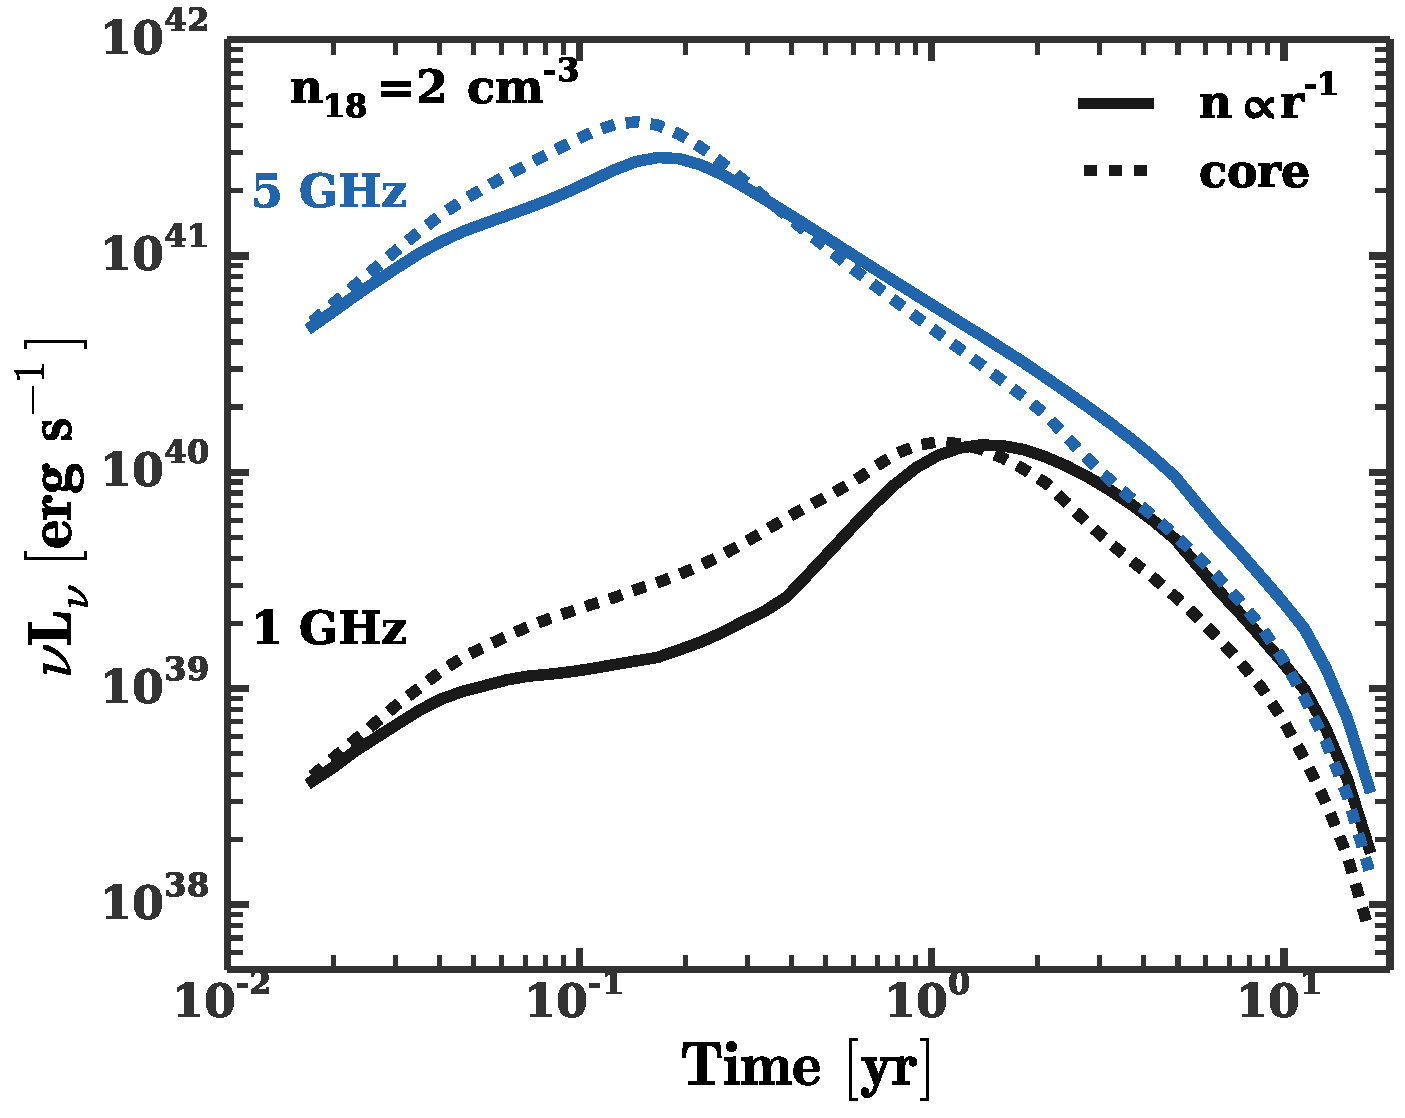
\includegraphics[width=8cm]{fig_cores.pdf}
  \caption{\label{fig:cores} Comparison of the light-curves for
    $n_{18}=2000$ and two different CNM gas density profiles: $n\sim
    r^{-1}$ and the core galaxy profile from \eqref{eq:cores} with
    $r_s=10^{18}$ cm and $n(r_s)=2000$, so that we can isolate the
    effect of the shape of the density profile. 4 pi correction}
\end{figure}


\subsection{Effects of viewing angle}


\section{Discussion}
\label{sec:disc}
{\bf AG -- Observational prescriptions and rates?}

\section{Summary and Conclusions}
\label{sec:conc}

\clearpage
  \footnotesize{
    \bibliographystyle{mnras}
    \bibliography{master}
  }

\end{document}
